\section{Desarollo packet pincer}

En esta sección veremos el funcionamiento de cada parte de la herramienta, la cual se ha llamado 'packet pincer' por el momento. Veremos qué y cuáles argumentos de consola acepta, como realiza la lectura de paquetes tanto en tiempo real como por trazas. A continuación se explicarán los diferentes pasos que llevan a cabo en el momento al analizar un paquete y como se realiza la generación de estadísticas. Finalmente, veremos como se realiza el etiquetado automático de los flujos y se escriben emiten los resultados.

El flujo principal de la aplicación se puede observar en la Figura \ref{fig:packetpincerexecution}. Como podemos ver, se van extrayendo paquetes mientras se encuentren disponibles. Cuando se obtiene uno, en caso de ser un paquete IPv4 fragmentado, se intenta reconstruir o se guarda en caso de no poder. A continuación, se comprueba si la herramienta soporta analizar el paquete indicado y, en caso afirmativo, acumula la información en el flujo de transporte respectivo. Finalmente, se 'cierran' los flujos antiguos, es decir, se emite la información relevante y a continuación se descarta el resto de información acumulada.

\begin{figure}[H]
  \begin{center}
    \centering
    \resizebox{!}{\dimexpr\textheight-2\baselineskip\relax}{%
      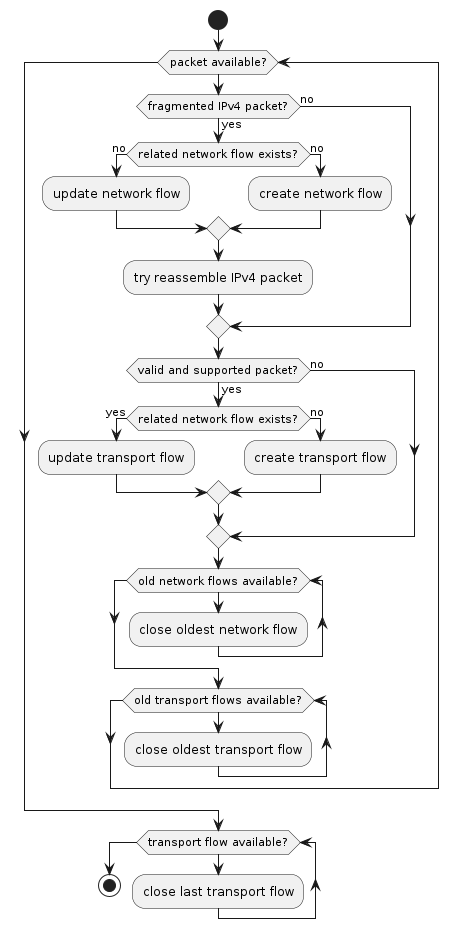
\includegraphics{plant_uml_diagrams/general_tool_loop.png}
    }
  \end{center}
  \caption{Flujo de la aplicación durante su ejecución}\label{fig:packetpincerexecution}
\end{figure}

\subsection{Argumentos y señales}

El programa está pensado para ser ejecutado desde el terminal. Debido a esto, hemos de definir que argumentos se pueden pasar al programa y hacer que este reaccione a señales del sistema operativo. Los argumentos suelen ser pasados desde el mismo comando utilizado para ejecutar el programa, siendo un ejemplo '\texttt{packet\_pincer \underline{help}}'. Las señales a su vez se pueden enviar utilizando una combinación de teclado como \texttt{CTRL+C} o utilizando otro programa.

Para hacer la gestión de los argumentos enviados por el terminal, se ha hecho uso de la librería (o 'crate', en la nomenclatura utilizada en Rust) clap \cite{Knapp_clap_2024}. Concretamente, se ha hecho uso de la funcionalidad 'derive', la cual permite expresar los argumentos a pasar como un tipo del lenguaje de forma declarativa. Adicionalmente, la librería añade diversas funcionalidades que mejoran la experiencia de usuario. A partir de nuestras definiciones, se muestran unas indicaciones de uso si se ejecuta \texttt{packet\_pincer --help} o si se pasan argumentos inválidos. Los argumentos definidos para el programa consisten en:

\begin{enumerate}
  \item Opcionalmente indicar si escribir los resultados generados en archivos (indicando su prefijo), en la salida estándar o no emitir nada.
  \item Opcionalmente indicar si un archivo en formato csv de las etiquetas que han de ponerse en los flujos. En caso de que se especifique este archivo y no haya etiqueta correspondiente, se generará una llamada 'benign'.
  \item Indicación del origen de los paquetes a analizar. Este puede ser 'offline' (a partir de una traza de red o un directorio de estas) u 'online' (a partir de una interficie de red).
\end{enumerate}

Respecto a las señales, se hace uso de la librería ctrlc \cite{controlc}. Esta permite detectar señales de interrupción enviadas por el usuario para interrumpir la ejecución de la aplicación. Si el programa no respondiese a estas señales, el sistema operativo terminaría el proceso directamente. Esto podría provocar la escritura parcial de los archivos, potencialmente corrompiéndolos. En caso de que se genere una señal de interrupción del programa, lo tratamos como que no hay más paquetes disponibles.

El código que se encarga de tratar estos puntos, se puede encontrar en \texttt{main.rs} en el anexo 2 o en el repositorio de GitHub.

\subsection{Lectura de paquetes}

\subsubsection{Librerias}

Para realizar la lectura de paquetes, tanto en tiempo real como a partir de archivos, se ha escogido hacer uso de la librería de rust 'pcap' \cite{rustpcap}, la cual a su vez hace uso internamente de otra llamada 'libpcap' la cual es desarrollada por el grupo tcpdump \cite{libpcap}. Dependiendo de si queremos leer paquetes desde un archivo o desde una interfaz de red, tendremos que utilizar una función de la API pública u otra para generar una instancia 'Capture'. 

\subsubsection{Detalles de implementación comunes}

A pesar de que la librería ofrece casi todas las funcionalidades que se requieren, no ofrece soporte para leer desde una lista de archivos, sino que hemos de leer de cada uno individualmente. Debido a esto, se ha creado la envoltura 'PacketCapture' disponible en \texttt{packet\_capture.rs} en el anexo 2 o en el repositorio de GitHub. En esta, se permite crear una instancia a partir de una ruta, que puede ser un archivo, un directorio o una interfaz de red. Adicionalmente, permite al usuario del módulo hacer una petición para procesar el siguiente paquete. Esto se hace a través de pasar una clausura que acepta un 'PacketOrigin' (ruta del archivo o nombre, interfaz), un 'LinkType' (el tipo de la capa de enlace \cite{linktypetcpdump}) y una referencia al paquete a tratar. La función de procesamiento extrae el siguiente paquete y llama a la clausura, devolviendo un valor afirmativo si se ha podido extraer un paquete o un valor negativo en caso de contrario.

Se hace uso de una clausura en vez de devolver una referencia al paquete debido a que el compilador no lo permitía. Después de investigar, esto era causado por el hecho que la librería pcap, dentro de la instancia 'Capture', tenía una referencia a un trozo de memoria. Al seguir manteniendo una referencia a la captura después de ejecutar la función, esto causaba que el compilador no pudiese garantizar que esta referencia fuese válida. En cambio, al pasar una clausura se puede asegurar a que se haga un uso correcto de la memoria al poder indicarlo en el prototipo de la función proporcionada por el usuario del módulo.

\subsubsection{Lectura de paquetes en tiempo real}

Para el caso de la lectura de paquetes en tiempo real, podemos hacer uso relativamente directo de la librería. En el momento de crear 'PacketCapture' creamos la instancia 'Capture' basada en una interficie de red. Cuando queremos procesar el siguiente paquete, pasamos la petición directamente a 'Capture' y a continuación ejecutamos la clausura. Si no hay errores, devolvemos un valor verdadero, indicando que hay potencialmente más paquetes válidos. En caso contrario, indicamos un valor negativo, indicando que probablemente no se puedan capturar más paquetes.

\subsubsection{Lectura de trazas de paquetes}

El caso de la lectura de trazas es más complicado. Debido a que se quiere admitir el poder leer de uno o varios archivos, es necesario hacer una mayor gestión adicional a la que nos proporciona la librería. Para esto, se han definido tres estructuras internas:
\begin{enumerate}
  \item \textbf{OwnedPacket}: Un paquete el cual 'posee' la memoria a la que hace referencia. A diferencia del que nos proporciona la librería pcap, no hace referencia a una sección de memoria que puede formar o no parte de otra mayor, permitiéndonos garantizar que las referencias a memoria son válidas.
  \item \textbf{FileCapture}: Una envoltura de una 'Capture' de la librería pcap con su ruta de origen y el siguiente paquete que se debe tratar extraído. Esto se hace para poder ordenar las diferentes 'FileCapture' según el tiempo de captura del paquete.
  \item \textbf{FileCaptureCollection}: Un conjunto de 'FileCapture'. Está estructurado en dos campos: un 'HashMap' de la librería estándar y en una cola de prioridad \cite{priority-queue}. El primero es utilizado para poder acceder en tiempo constante a cualquier 'FileCapture' a partir de su ruta y el segundo para tener una lista ordenada de más a menos antiguo del siguiente paquete a analizar. Esto es necesario debido a que hay algunos conjuntos de datos contienen archivos que se solapan en el tiempo.
\end{enumerate}

(explicar el proceso de creación)

(explicar el proceso de obtención del siguiente paquete)

\subsection{Extensión de libreria de código abierto para la decodificación de paquetes}

Por hacer

\subsection{Defragmentación IPv4}

Por hacer

\subsection{Separación de flujos}

Por hacer

\subsection{Generación de estadísticas}

Por hacer

\subsection{Escritura y etiquetado de flujos}

Por hacer

